\documentclass[18pt]{beamer}
\usetheme{Madrid}
\usepackage{alltt}
\usepackage{graphics}
\usepackage{listings}
\usepackage{url}
\usepackage{verbatim}
\usepackage{xcolor}

\lstset{language=C++,numbersep=1pt,identifierstyle=\color{blue!50!black},commentstyle=\color{yellow!50!black},xleftmargin=7pt,numberblanklines=false,numberstyle=\color{red!60!black},numbers=left,basicstyle=\tiny\ttfamily,keywordstyle=\color{green!60!black}\bfseries,stringstyle=\color{red!80!black}}
\lstset{frame=shadowbox, rulesepcolor=\color{blue},breaklines=true,numbersep=5pt,basicstyle=\small\ttfamily}
\newcommand{\lstlistingwithnumber}[3]{
\begin{center}
\lstinputlisting[linerange={#1-#2},firstnumber=#1]{#3}
\end{center}
}

\newcommand{\centeredlargetext}[3]{
{
\setbeamertemplate{background}{}
\setbeamertemplate{navigation symbols}{}
\setbeamercolor{background canvas}{bg={#1}}
\color{#2}
\begin{frame}[plain]
\fontsize{36pt}{36pt}\selectfont
\center
\begin{center}
{#3}
\end{center}
\end{frame}
}}

\newcommand{\centeredhugetext}[3]{
{
\setbeamertemplate{navigation symbols}{}
\setbeamercolor{background canvas}{bg={#1}}
\fontsize{72pt}{72pt}\selectfont
\color{#2}
\begin{frame}[plain]
\center
\begin{center}
{#3}
\end{center}
\end{frame}
}}


\begin{document}

\title[ANTsMM]{Multi-modality processing with \newline Advanced Normalization
  Tools (ANTs)}
\subtitle[ANTsMM]{Modern data fusion strategies}
\institute[PICSL]{Brian Avants, PICSL and the ANTs Development Team}
\date

\begin{frame}
\titlepage
\end{frame}


{
\setbeamertemplate{navigation symbols}{}
\begin{frame}[plain]
\center
\begin{center}
This presentation is copyrighted by\\
The \textbf{ANTs software consortium}\\
\bigskip
distributed under the\\
\textbf{Creative Commons by Attribution License 3.0}\\
\url{http://creativecommons.org/licenses/by/3.0}\\
\end{center}
\end{frame}
}


% \begin{frame}
%  \tableofcontents[hideallsubsections]
% \end{frame}

% \setbeamertemplate{background}{
\includegraphics[width=\paperwidth]{../figures/ITKv4_transparent}}
\setbeamertemplate{background}{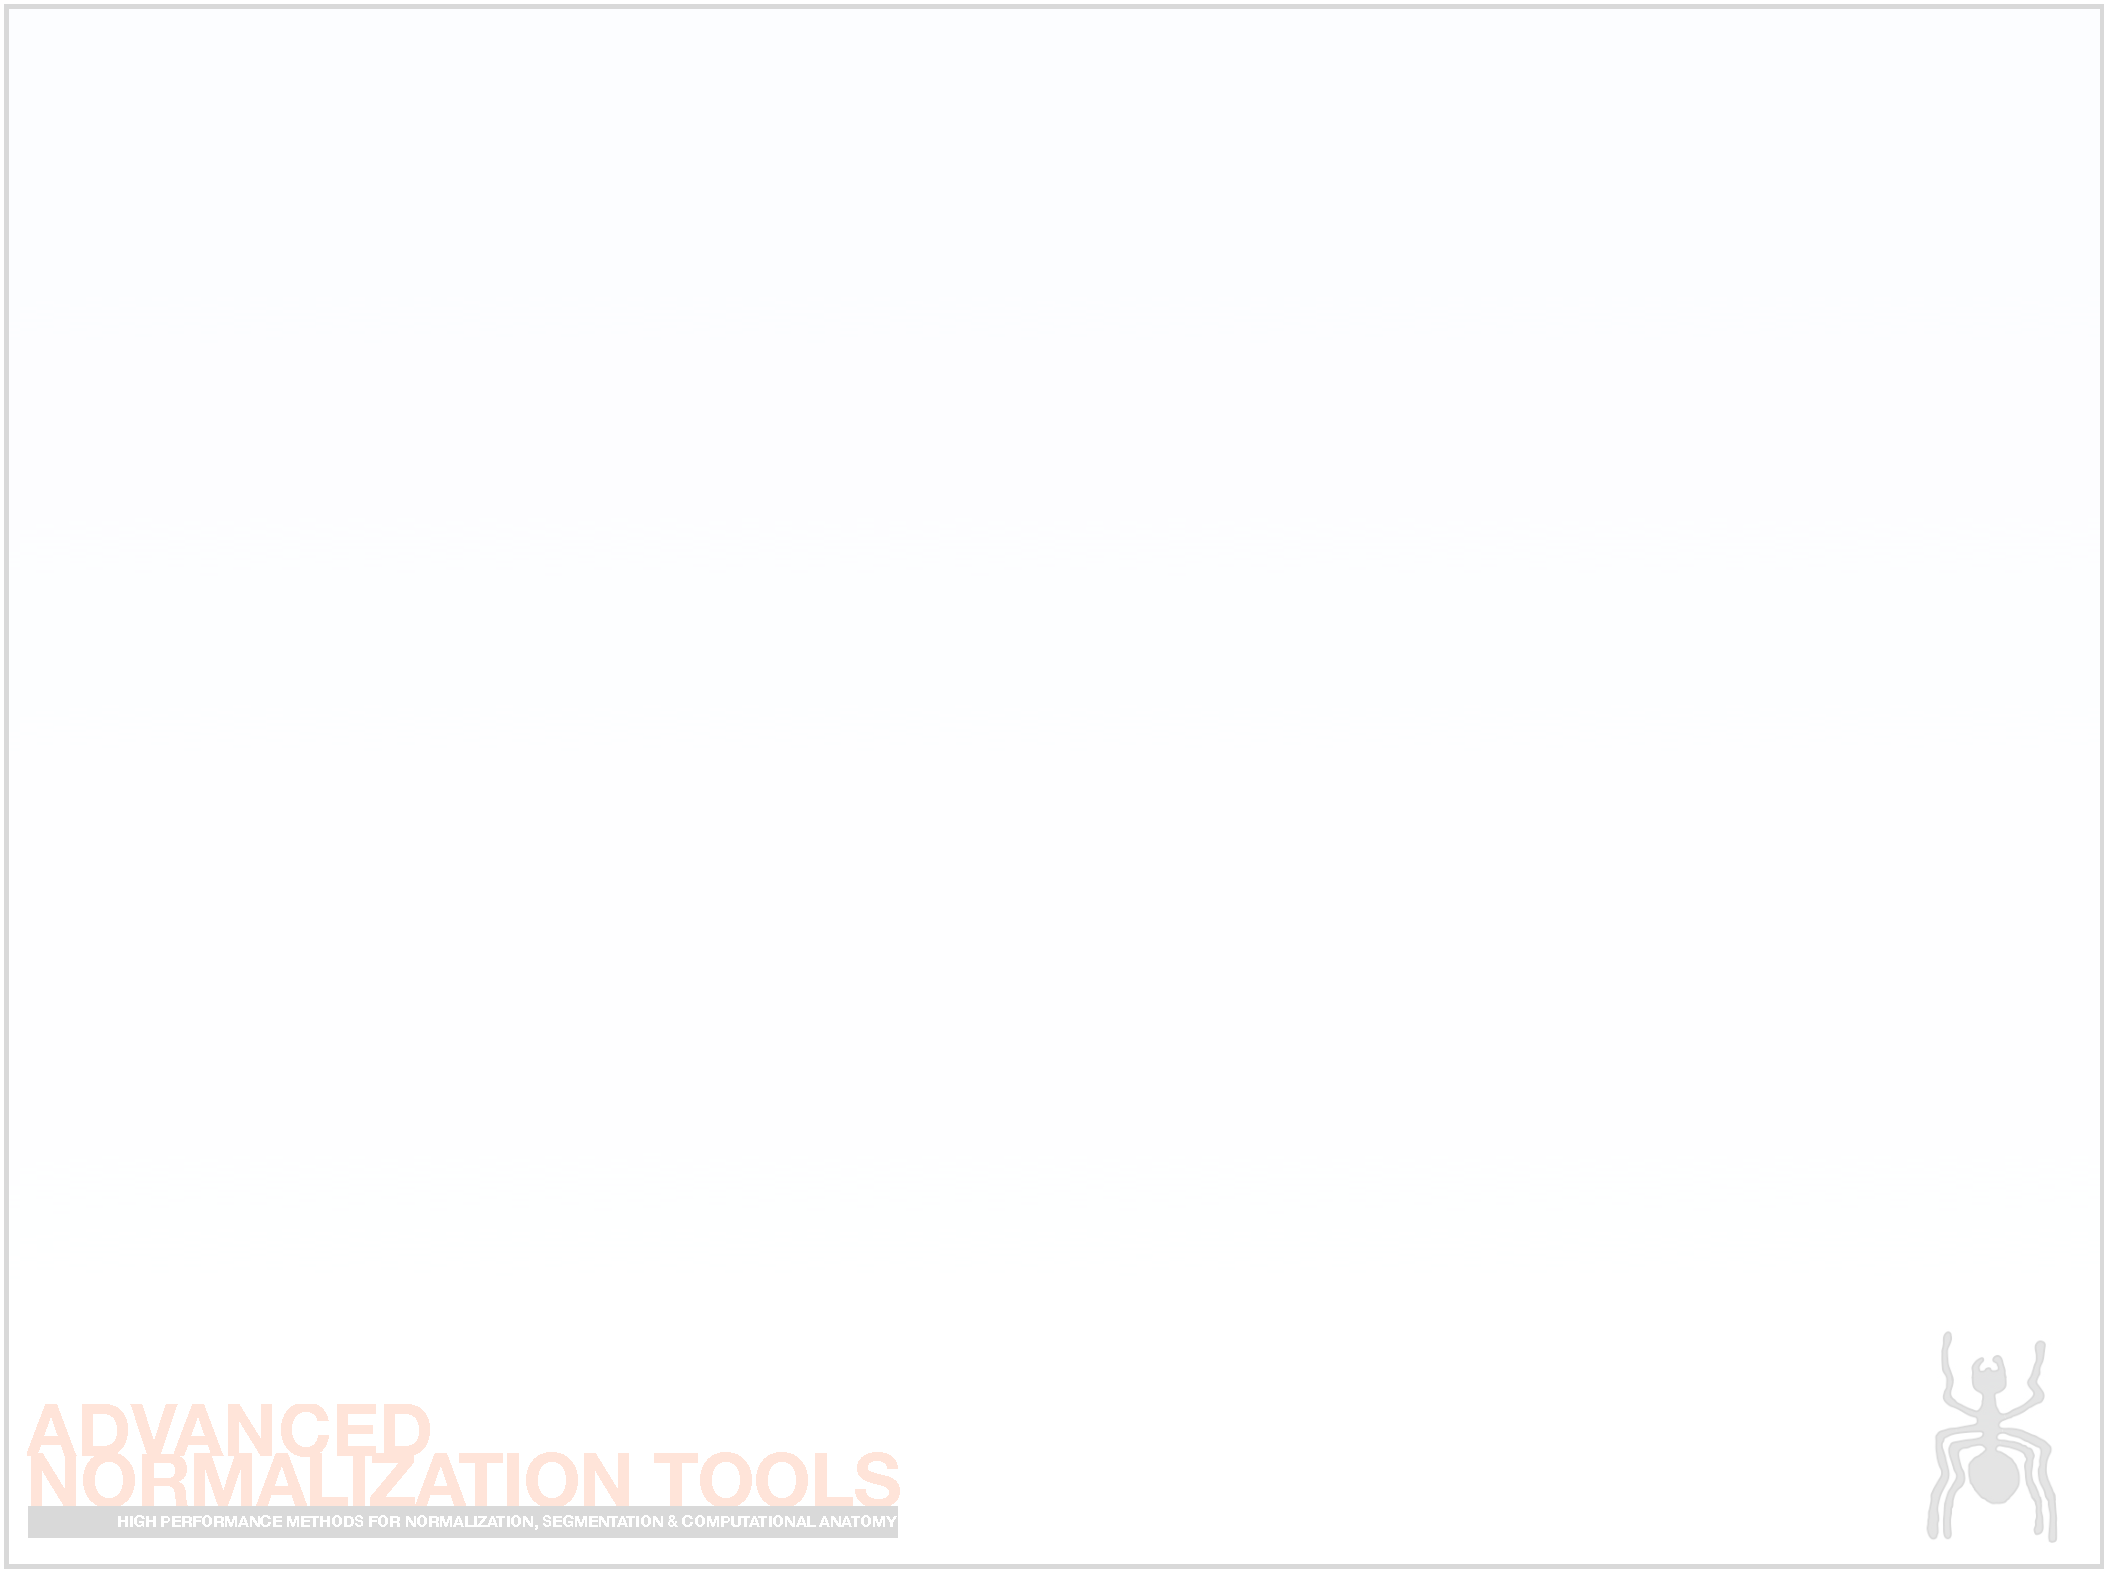
\includegraphics[width=\paperwidth]{../figures/ants_background2.pdf}}


\begin{frame}
\frametitle{People}
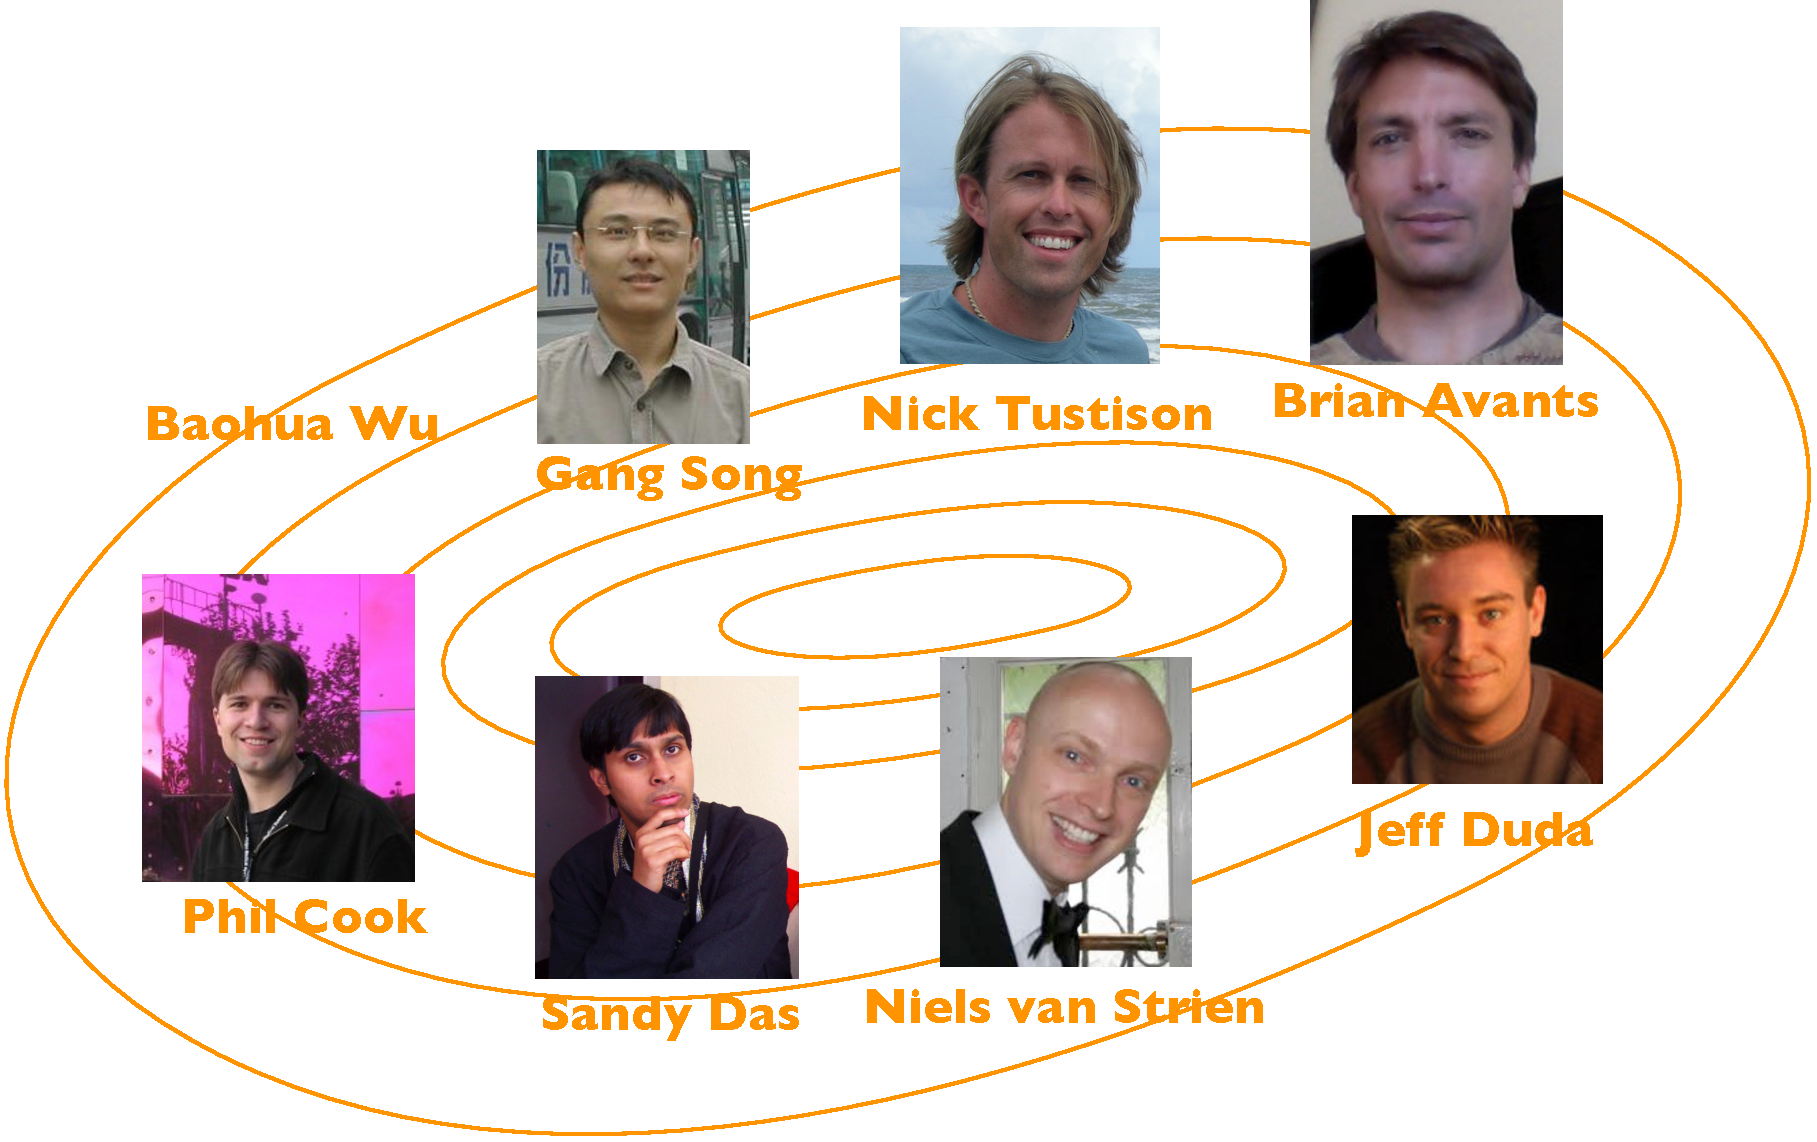
\includegraphics[width=\paperwidth]{../figures/ants_contributors.pdf}
\end{frame}

\begin{frame}
\frametitle{History: Theory}
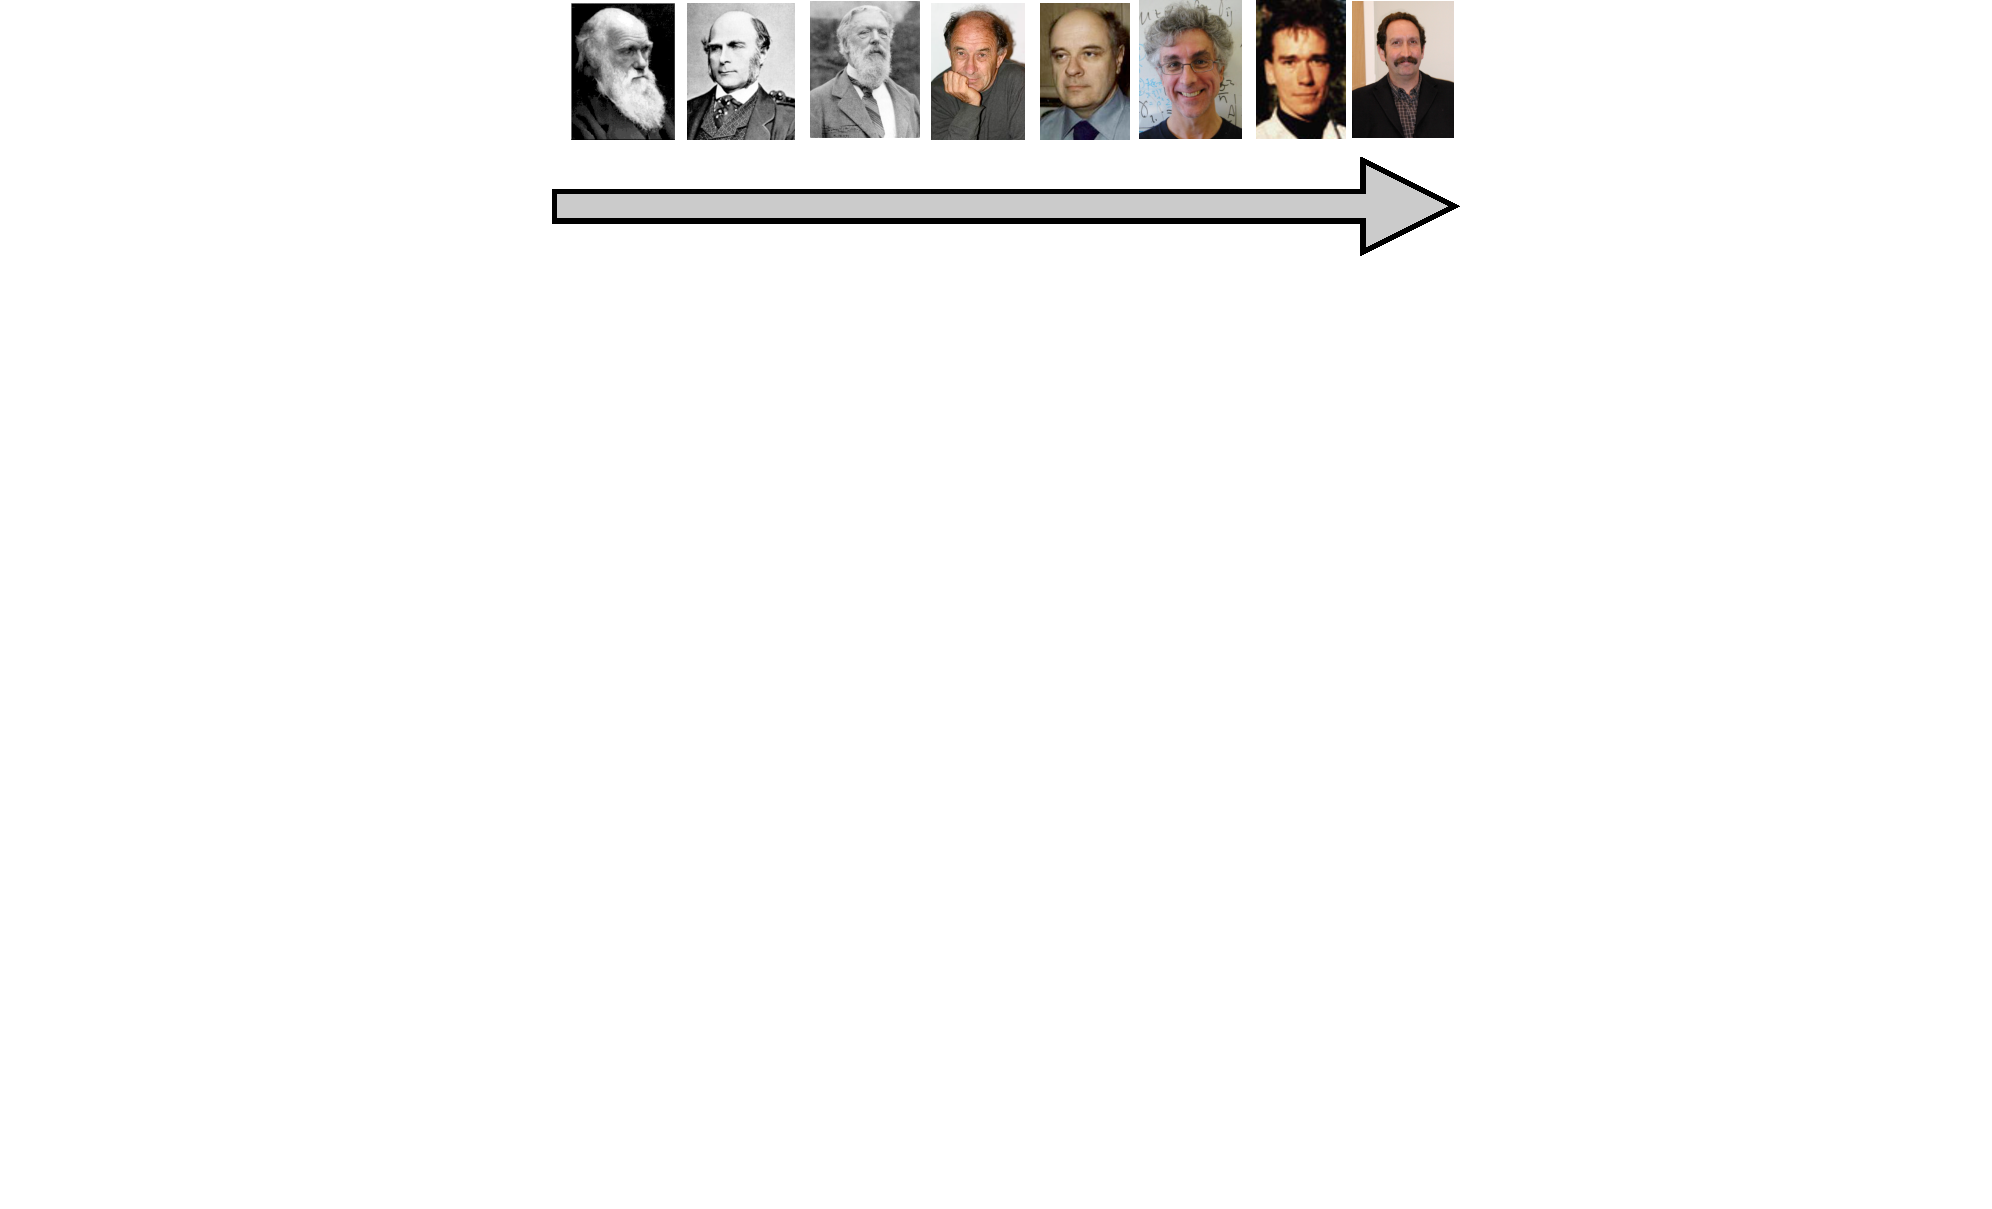
\includegraphics[width=\paperwidth]{../figures/ants_history_t.pdf}
\end{frame}

\begin{frame}
\frametitle{History: Implementation}
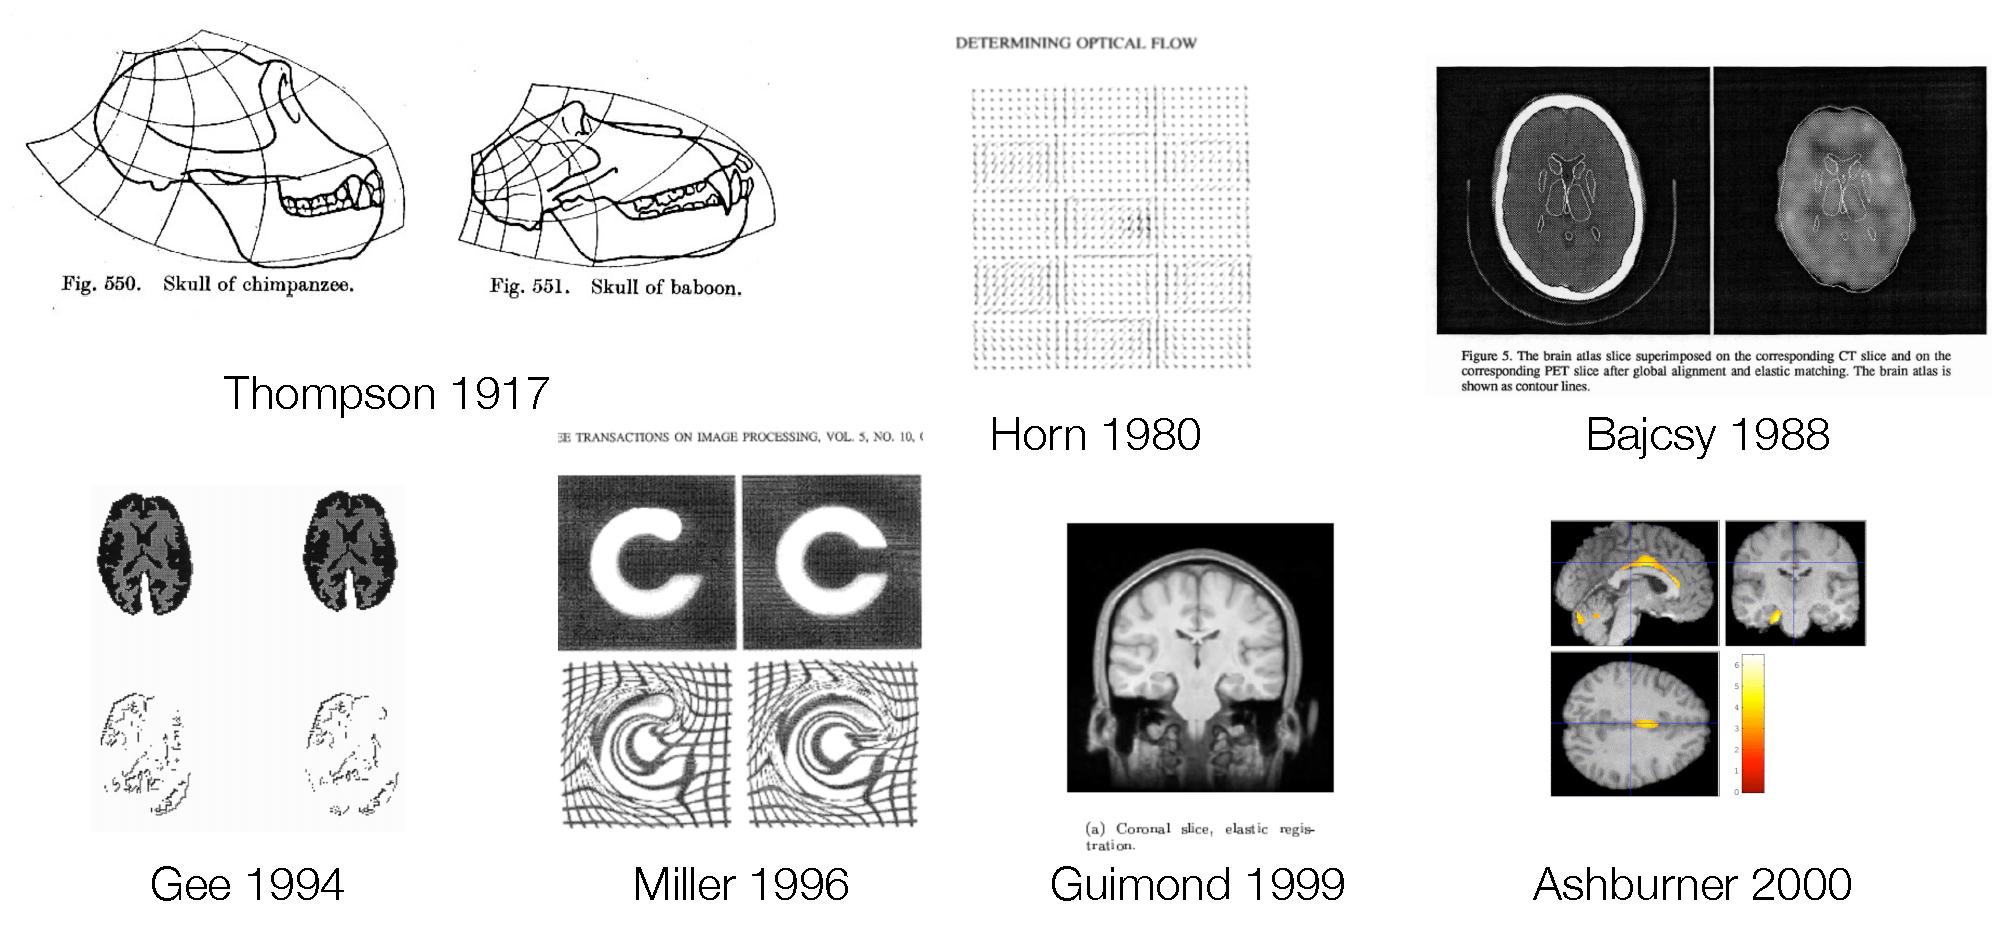
\includegraphics[width=4.75in]{../figures/ants_history.pdf}
\end{frame}

\begin{frame}
\frametitle{Download ANTs binaries.}
Go to:
\newline
\newline
\href{http://sourceforge.net/projects/advants/files/}{link: \textcolor{blue}{ANTS release files}}
\newline
\newline
 You will see folders for documentation, code, binaries.
\newline
\newline
From the folder ANTS, select a specific release, e.g.:
\newline
\newline
\href{http://sourceforge.net/projects/advants/files/ANTS/ANTS_1_9\_x/}{link: \textcolor{blue}{1\_9\_x binaries}}
\end{frame}

\begin{frame}
\frametitle{Install ANTs from source: Requires  git/svn cmake, C++}
open a terminal window and make a new directory.  call it ANTs.

$>$ mkdir ANTs

$>$ cd ANTs

then type

$>$ svn checkout https://advants.svn.sourceforge.net/svnroot/advants
ANTS

$>$  mkdir bin

$>$  cd bin/

$>$  ccmake ../ANTS/trunk/

\end{frame}

\begin{frame}
\frametitle{Install ANTs from source: Requires  git/svn, cmake, C++}

then, in cmake, type “c” and then “g”  then exit back to the
terminal.   then:

$>$  make -j 4

and wait a while.

If there is an error like  ``cannot find 'some ITK file' `` then try
this:
\newline
\newline
from the bin directory, cd into ITKv4 , then type:

$>$  git pull origin master

that will update ITK.

you can then try 'make -j 4' again.
\end{frame}

\begin{frame}
\frametitle{Overview:  Program $+$ brief description 1}
%ants overview of tools :  multivariate registration, segmentation, bias correction, template building and image-math 
\begin{tiny}
{
\begin{table}
\begin{tabular}{|p{2.0cm}|p{2.5cm}|p{3cm}|p{3cm}|}
\hline
        Tool Name                                     & Description                                                                                                                                                    & Highlights                                                                                                         & Primary Reference                                                                                                                                                                                   \\ \hline
        ANTS                                          & Interface to a
variety of registration algorithms & Best performing normalization algorithm in multiple different studies.                                             & A reproducible evaluation of ANTs similarity metric performance in brain image registration                                                                                                         \\ 
        antsRegistration                              & ITKv4 update to ANTS.                                                    & Takes full advantage of multi-core processing.                                                                     & A unified registration framework for ITK, WBIR 2012.                                                                                                                                                \\ 
        Atropos                                       & Multivariate probabilitic EM segmentation                                                                                                                      & Can integrate information from multiple modalities and has a DTI-specific likelihood.                              & An open source multivariate framework for n-tissue segmentation with evaluation on public data.                                                                                                     \\ 
        N4BiasFieldCorr...                         & Novel
inhomogeneity field correction
method                                                                                                                   
& Considered new standard in bias correction by much of the medical imaging community.                       & N4ITK: improved N3 bias correction.                                                                                                                                                                 \\ 
        ImageMath                                     & Basic operations on images.                                                                                                                                    & Works on 2D, 3D, 4D images.                                                                                        & ---                                                                                                                                                                                             \\ 
        buildtemplateparallel                         & Optimal template construction in the diffeomorphic space.                                                                                                      & Used as a standard evaluation target for new template construction methodology.  New multimodality implementation. & The optimal template effect in hippocampus studies of diseased populations                                                                                                                          \\ 
\hline
\end{tabular}
\end{table}
}
\end{tiny}
\end{frame}


\begin{frame}
\frametitle{Overview:  Program $+$ brief description 2}
%ants overview of tools :  multivariate registration, segmentation, bias correction, template building and image-math 
\begin{tiny}
{
\begin{table}
\begin{tabular}{|p{2.1cm}|p{2.4cm}|p{3cm}|p{3cm}|}
\hline
        Tool Name                                     & Description                                                                                                                                                    & Highlights                                                                                                         & Primary Reference                                                                                                                                                                                   \\ \hline
        WarpImageMultiTrans... & Concatenates ANTS/ITK transforms                                                                                                                               & Can string together a series of N transforms to minimize interpolation error and resample.                         & ---                                                                                                                                                                                             \\ 
        antsApplyTransforms & Concatenates ANTS/ITK transforms                                                                                                                               & Can string together a series of N transforms to minimize interpolation error and resample.                         & ---                                                                                                                                                                                             \\ 
        KellyKapowski                                 & Cortical thickness estimation based on volumetric imagery + probabilistic segmentation                                                                         & The only multi-platform volumetric alternative to Freesurfer                                                       & Registration based cortical thickness measurement.                                                                                                                                                  \\ 
        sccan                                         & Multivariate dimensionality reduction                                                                                                                          & New tools with lots of potential for improving detection power in medical imaging.                                 & Dementia induces correlated reductions in white matter integrity and cortical thickness: a multivariate neuroimaging study with sparse canonical correlation analysis.                              \\ 
        antsMotionCorr                                & Motion correction + template construction methods for 4D images                                                                                                & Simple flexible rigid, affine, deformable motion correction for (mostly) functional data.                          & Estimation of perfusion and arterial transit time in myocardium using free-breathing myocardial arterial spin labeling with navigator-echo (not ideal but the only relevant one currently existing) \\
\hline
\end{tabular}
\end{table}
}
\end{tiny}
\end{frame}

\begin{comment}
{
\begin{frame}
\frametitle{Overview: Program $+$ highlight.}
%ants overview of tools :  multivariate registration, segmentation, bias correction, template building and image-math 
\begin{tiny}
{
\begin{table}
\begin{tabular}{|l|l|l|}
\hline
        Tool Name                                     & Highlights                                                                                                         & Primary Reference                                                                                                                                                                                   \\ \hline
        ANTS                                          & Best performing normalization algorithm in multiple different studies.                                             & A reproducible evaluation of ANTs similarity metric performance in brain image registration                                                                                                         \\ 
        antsRegistration                              & Takes full advantage of multi-core processing.                                                                     & A unified registration framework for ITK, WBIR 2012.                                                                                                                                                \\ 
        Atropos                                       & Can integrate information from multiple modalities and has a DTI-specific likelihood.                              & An open source multivariate framework for n-tissue segmentation with evaluation on public data.                                                                                                     \\ 
        N4BiasFieldCorrection                         & Considered new
standard in bias correction by much of the medical imaging community & N4ITK: improved N3 bias correction.                                                                                                                                                                 \\ 
        ImageMath                                     & Works on 2D, 3D, 4D images.                                                                                        & ---                                                                                                                                                                                             \\ 
        buildtemplateparallel                         & Used as a standard evaluation target for new template construction methodology.  New multimodality implementation. & The optimal template effect in hippocampus studies of diseased populations                                                                                                                          \\ 
        WarpImageMultiTransform & Can string together a series of N transforms to minimize interpolation error and resample.                         & ---                                                                                                                                                                                             \\ 
        antsApplyTransforms & Can string together a series of N transforms to minimize interpolation error and resample.                         & ---                                                                                                                                                                                             \\ 
        KellyKapowski                                 & The only multi-platform volumetric alternative to Freesurfer                                                       & Registration based cortical thickness measurement.                                                                                                                                                  \\ 
        sccan                                         & New tools with lots of potential for improving detection power in medical imaging.                                 & Dementia induces correlated reductions in white matter integrity and cortical thickness: a multivariate neuroimaging study with sparse canonical correlation analysis.                              \\ 
        antsMotionCorr                                & Simple flexible rigid, affine, deformable motion correction for (mostly) functional data.                          & Estimation of perfusion and arterial transit time in myocardium using free-breathing myocardial arterial spin labeling with navigator-echo (not ideal but the only relevant one currently existing) \\
\hline
\end{tabular}
\end{table}
}
\end{tiny}
\end{frame}


\begin{frame}
\frametitle{Overview: Program $+$ reference.}
%ants overview of tools :  multivariate registration, segmentation, bias correction, template building and image-math 
\begin{tiny}
{
\begin{table}
\begin{tabular}{|l|l|l|}
\hline
        Tool Name                                     & Primary Reference                                                                                                                                                                                   \\ \hline
        ANTS                                          & A reproducible evaluation of ANTs similarity metric performance in brain image registration                                                                                                         \\ 
        antsRegistration                              & A unified registration framework for ITK, WBIR 2012.                                                                                                                                                \\ 
        Atropos                                       & An open source multivariate framework for n-tissue segmentation with evaluation on public data.                                                                                                     \\ 
        N4BiasFieldCorrection                         & N4ITK: improved N3 bias correction.                                                                                                                                                                 \\ 
        ImageMath                                     & ---                                                                                                                                                                                             \\ 
        buildtemplateparallel                         & The optimal template effect in hippocampus studies of diseased populations                                                                                                                          \\ 
        WarpImageMultiTransform & ---                                                                                                                                                                                             \\ 
        antsApplyTransforms & ---                                                                                                                                                                                             \\ 
        KellyKapowski                                 & Registration based cortical thickness measurement.                                                                                                                                                  \\ 
        sccan                                         & Dementia
induces correlated reductions in white matter integrity and cortical
thickness ...                              \\ 
        antsMotionCorr                                & Estimation of perfusion and arterial transit time in myocardium using free-breathing myocardial arterial spin labeling with navigator-echo (not ideal but the only relevant one currently existing) \\
\hline
\end{tabular}
\end{table}
}
\end{tiny}
\end{frame}
}
\end{comment}


\begin{frame}
\frametitle{Scripting for large-scale studies}
\Large ANTs is for scripting!
\begin{alltt} 
 \#! /usr/bin/bash \newline
 echo ANTs likes short bash scripts
\end{alltt}
\begin{alltt} 
\#! /usr/bin/perl \newline
print "Longer scripts should use perl";
\end{alltt}
\begin{alltt} 
\#! /usr/bin/Rscript \newline
print( paste( "but ANTs prefers'',''{\bf R}'' ) )
\end{alltt}
\end{frame}

\begin{frame}
\frametitle{The Basic Toolset}
 \textcolor{blue}{Registration: Data is in Examples/Data} 
\begin{alltt}
ANTS 2 -m  CC[r16slice.nii.gz,r64slice.nii.gz,1,4] \newline
 -t SyN[0.25]  -r Gauss[3,0] -o TEST -i 50x40x30
\end{alltt}
\textcolor{blue}{Segmentation}
\begin{alltt}
Atropos -d 2 -a r16slice.nii.gz -x r16mask.nii.gz \newline
-m [0.1,1x1]   -c [10,0]  -i kmeans[3]\newline
-o [Output.nii.gz,Output\_prob\_\%02d.nii.gz]
\end{alltt}
\textcolor{blue}{Template building}
\begin{alltt}
 bash buildtemplateparallel.sh -d 3 -m 30x50x20 \newline 
-t GR  -s CC -c 1 -o OutPrefix  *ImageName*T1x.nii.gz
\end{alltt}
\end{frame}
% ants-essential tools:  a mapping, a segmentation, a template and then label-guided and multivariate versions of these.  


\begin{frame}
\frametitle{Basic applications}
\begin{itemize}
\item Quantify changes in cortical thickness in an individual.
\pause 
\item Perform a template-based study of thickness, gray matter
  probability, FA, rs connectivity ... 
\pause
\item Identify multivariate relationships between modalities and
  predictors.
\pause
\item Single-subject BOLD fmri study of resting state connectivity.
\pause
\item Asymmetry study of neuroanatomy.
\pause
\item In general, optimal dimensionality reduction to increase detection power.  
\end{itemize}
\end{frame}



\begin{frame}
\frametitle{Segmenting anatomy from an image}
See  examples/segmentation\_example.sh
\lstinputlisting{segmentation_example_input.tex}
\begin{center}
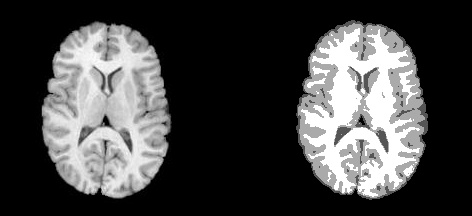
\includegraphics[width=3.in]{../figures/r64sliceseg.jpg}
\end{center}
\end{frame}

\begin{frame}
\frametitle{Multivariate anatomical segmentation}
See  examples/segmentation2\_example.sh
\lstinputlisting{segmentation2_example_input.tex}
\begin{center}
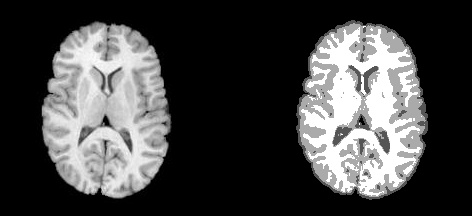
\includegraphics[width=3.in]{../figures/r64sliceseg2.jpg}
\end{center}
 \end{frame}

\begin{frame}
\frametitle{Meaning of parameters}
What happens when i vary each parameter?
\begin{alltt}
-i priorprobabilityimages[3, inprob\%02d.nii.gz, k ]  \newline
~~~~~vs.  \newline
-i kmeans[ k ]
\end{alltt}
\begin{center}
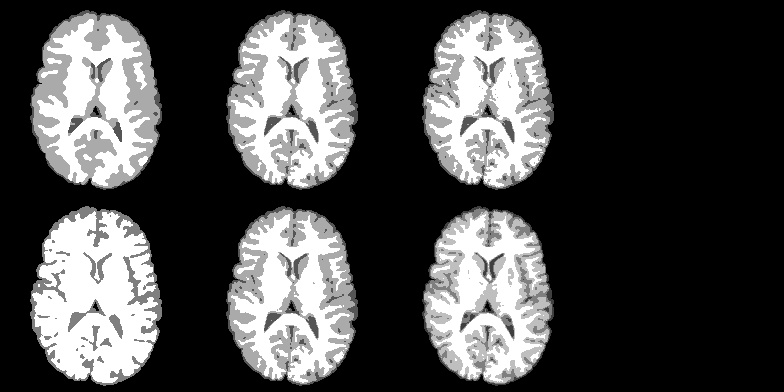
\includegraphics[width=3.in]{../figures/r64segparams.jpg}\newline
Vary MRF param and K in k-means.
\end{center}
\end{frame}

\begin{frame}
\frametitle{Cortical thickness from imaging data}
See  examples/thickness\_example.sh
\lstinputlisting{thickness_example_input.tex}
\begin{center}
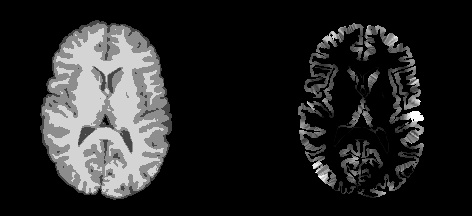
\includegraphics[width=4.in]{../figures/r64thickness.jpg}
\end{center}
{\bf Can vary smoothness, priors on thickness, etc.  See help. }
\end{frame}

\centeredlargetext{white}{blue}{
But isn't ANTs all about normalization?
}

\centeredlargetext{white}{blue}{
But isn't ANTs all about registration?
}

\centeredlargetext{white}{blue}{
But isn't ANTs all about mapping?
}

\centeredlargetext{white}{blue}{
But isn't ANTs all about transformations and templates?
}

\begin{frame}
\frametitle{Template-based transformations}
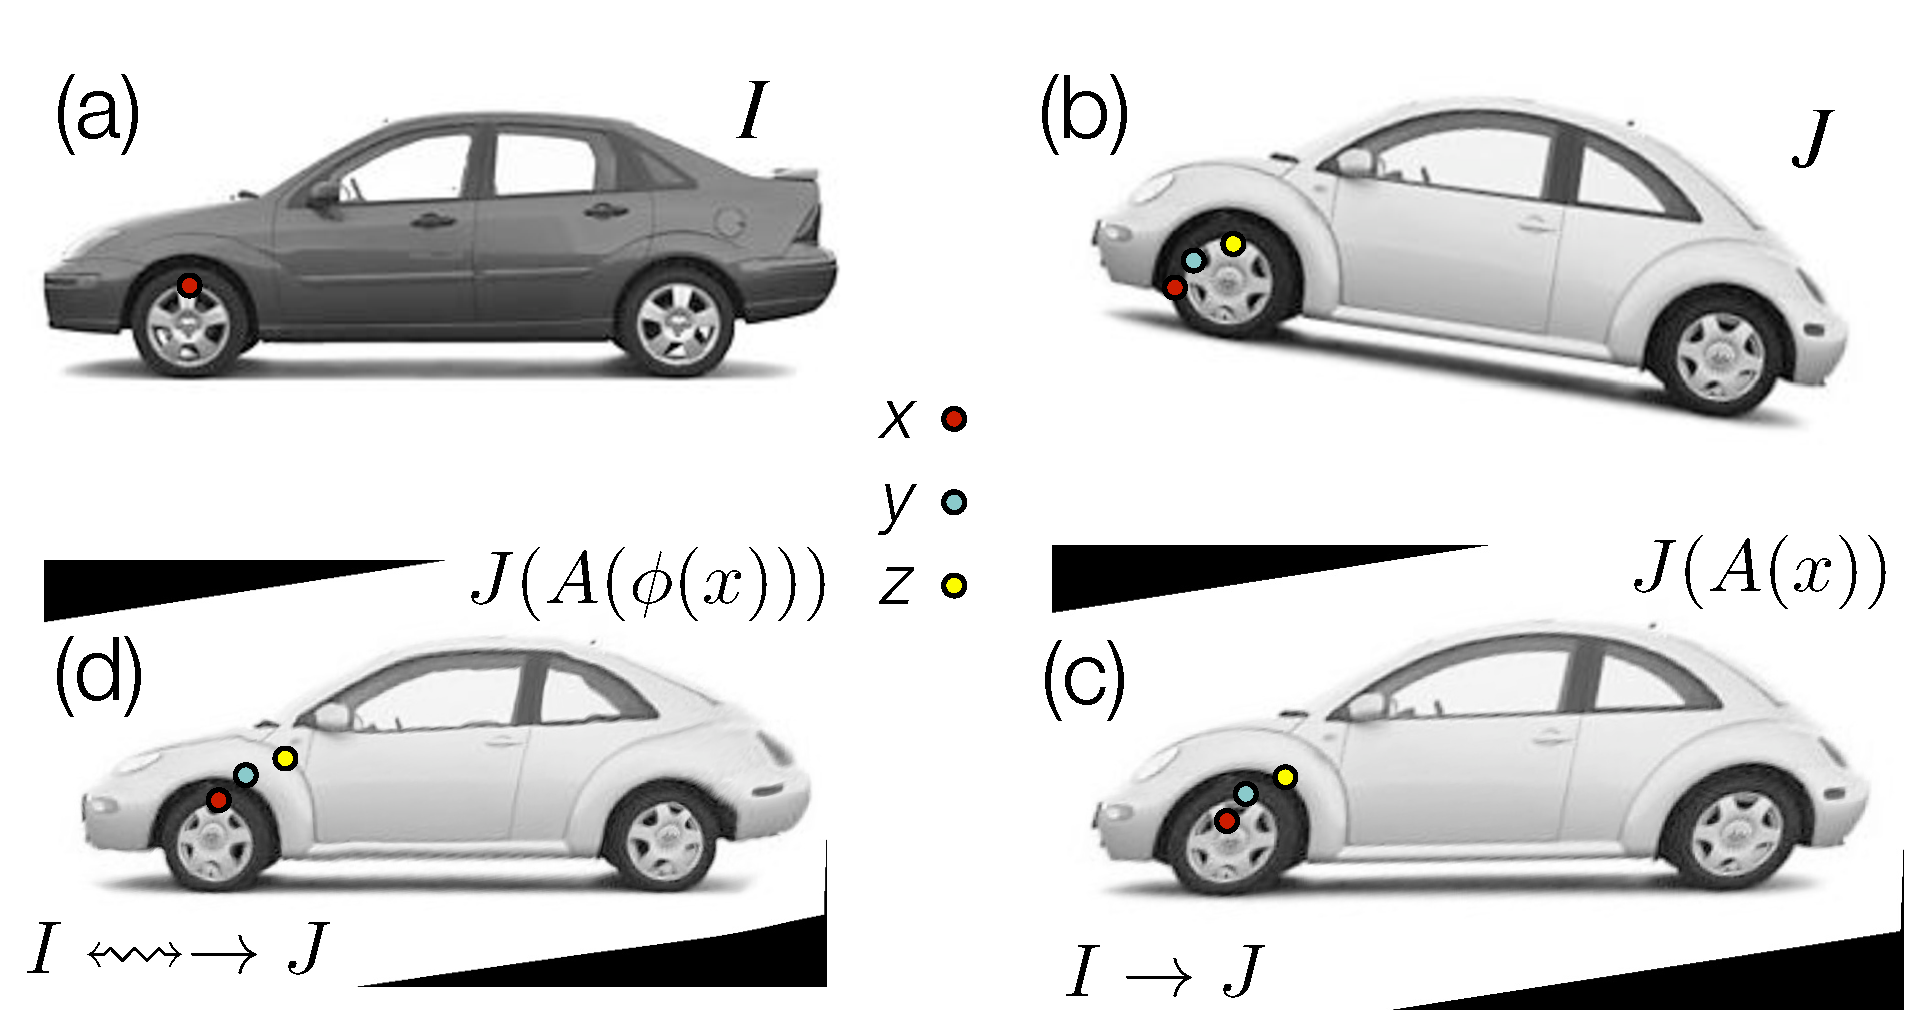
\includegraphics[width=4.5in]{../figures/car_example.pdf}
\end{frame}

\begin{frame}
\frametitle{How did we compute that transformation?}
\lstinputlisting{cars.sh}
\end{frame}


\begin{frame}
\frametitle{Mapping two images}
See  examples/registration\_example.sh
\lstinputlisting{registration_example_input.tex}
\end{frame}

\begin{frame}
\frametitle{Mapping two images}
\begin{center}
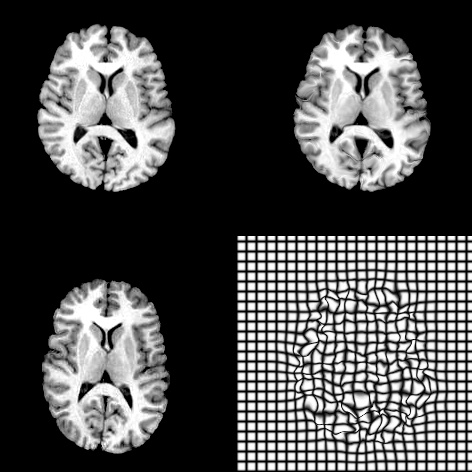
\includegraphics[width=3.in]{../figures/r64registration.jpg}
\end{center}
{\bf Can vary smoothness, metrics, etc.  See help. }
\end{frame}

\begin{frame}
\frametitle{Meaning of parameters}
\Large What happens when i vary each parameter?
\begin{itemize}
\item Robustness increases with regularization ( -r Gauss[6,3] $>$ -r
  Gauss[3,0] )
\pause
\item Flexibility decreases with regularization ( -r Gauss[6,3] $<$ -r
  Gauss[3,0] )
\pause
\item Robustness increases with correlation window ( -m CC[ . , . , 1
  , 4 ] $<$  -m CC[ . , . , 1
  , 6 ]  )  but computation time also increases
\pause
\item Details matter:  pre-processing, feature extraction, etc. 
\pause
\item Successful affine step is essential!!
\pause
\item Step-size increases stability but slows convergence ( SyN[ 0.1 ]
  more stable than SyN[ 0.25 ] ).
\end{itemize}
\end{frame}

\begin{frame}
\frametitle{Check the affine mapping between two images}
See  examples/registration\_affine\_example.sh
\lstinputlisting{registration_affine_example_input.tex}
\begin{center}
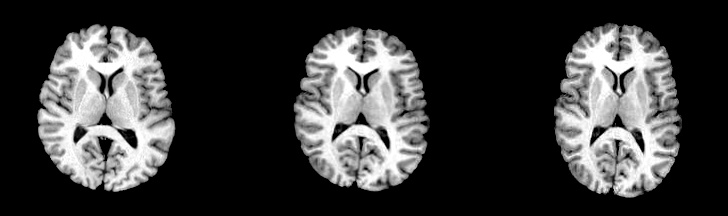
\includegraphics[width=4in]{../figures/r64registrationaffine.jpg}\newline
{\bf fixed   versus affinely registered image versus original moving}
\end{center}
\end{frame}

\begin{frame}
\frametitle{Coordinates of computation time}
\begin{Large}
\begin{itemize}
\item 2D 256$^2$ pixels intensity difference (MSQ) registration
  $\approx$ \textcolor{red}{30 seconds}
\pause
\item 3D 256$^3$ voxels correlation-8 ( CC[ . , . , 1,
8] ) could take \textcolor{red}{3 days} if you use full-resolution and the images are
very different.
\pause
\item  or it could take \textcolor{red}{15 minutes} if you use low-resolution and the
  images are very similar.
\end{itemize}
\end{Large}
\end{frame}

\begin{frame}
\frametitle{Multiple metrics driving registration}
% face example and why we use LMs @ the same time as data 
See  examples/registration\_mm\_example.sh
\lstinputlisting{registration_mm_example_input.tex}
\begin{center}
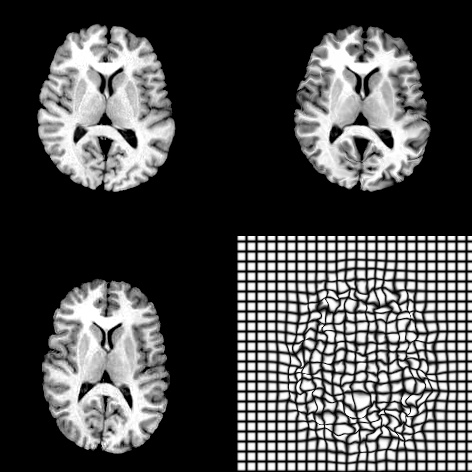
\includegraphics[width=4in]{../figures/r64registrationmm.jpg}\newline
{\bf fixed versus ... }
\end{center}
\end{frame}


\begin{frame}
\frametitle{Landmark-based registration 1}
% Schoenemann examples affine + bspline 
% face example and why we use LMs @ the same time as data 
\begin{center}
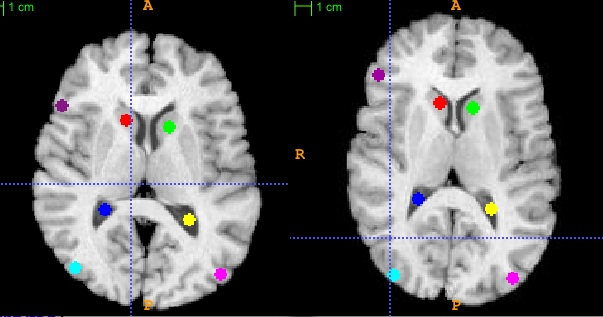
\includegraphics[width=4in]{../figures/landmarks.jpg}\newline
{\bf .}
\end{center}
\end{frame}

\begin{frame}
\frametitle{Landmark-based registration 2}
% Schoenemann examples affine + bspline 
% face example and why we use LMs @ the same time as data 
See  examples/registration\_lm\_example.sh
\lstinputlisting{registration_lm_example_input.tex}
\end{frame}


\begin{frame}
\frametitle{Landmark-based registration 3}
\begin{center}
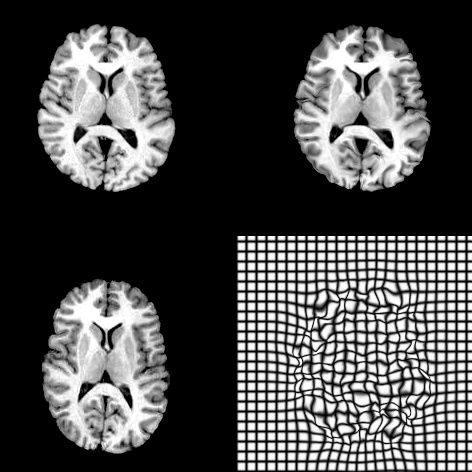
\includegraphics[width=4in]{../figures/r64registrationlm.jpg}\newline
{\bf fixed versus ... }
\end{center}
\end{frame}


\begin{frame}
\frametitle{Other Landmark-based registration tools}
\begin{itemize}
\item for 3D
\item ANTSUseLandmarkImagesToGetAffineTransform lm1.nii.gz lm2.nii.gz affine outaffine.txt
\item ANTSUseLandmarkImagesToBSplineDisplacementField outLMWarp.nii.gz
  10x10x10 6 3 0
\item Then use WarpImageMultiTransform / antsApplyTransform to apply
  the warp to the relevant image.
\end{itemize}
\end{frame}


\begin{frame}
\frametitle{Template construction}
group studies 
\end{frame}

\begin{frame}
\frametitle{Templates for asymmetry analysis}
chimpanzee cortical thickness 
\end{frame}

\begin{frame}
\frametitle{Templates for all modalities}
what is common?  brain
\end{frame}

\begin{frame}
\frametitle{Longitudinal analysis with ANTs}
look at data ... good rigid
\end{frame} 

\begin{frame}
\frametitle{Time series / rsfMRI analysis with ANTs}
See  examples/motioncorr\_example.sh
\lstinputlisting{motioncorr_example_input.tex}
\begin{itemize}
\item mi --- mutual information metric 
\pause
\item Rigid --- use rigid map to the average with gradient step 0.05
\pause
\item other params --- smoothing, scale estimation, iterations ... 
\end{itemize}
\end{frame}

\begin{frame}
\frametitle{Time series / rsfMRI analysis with ANTs}
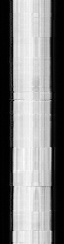
\includegraphics[width=2in]{../figures/rsfmri_discon.jpg}
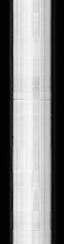
\includegraphics[width=2in]{../figures/rsfmri_smooth.jpg}
\end{frame}

\begin{frame}
\frametitle{Time series / rsfMRI analysis with ANTs}
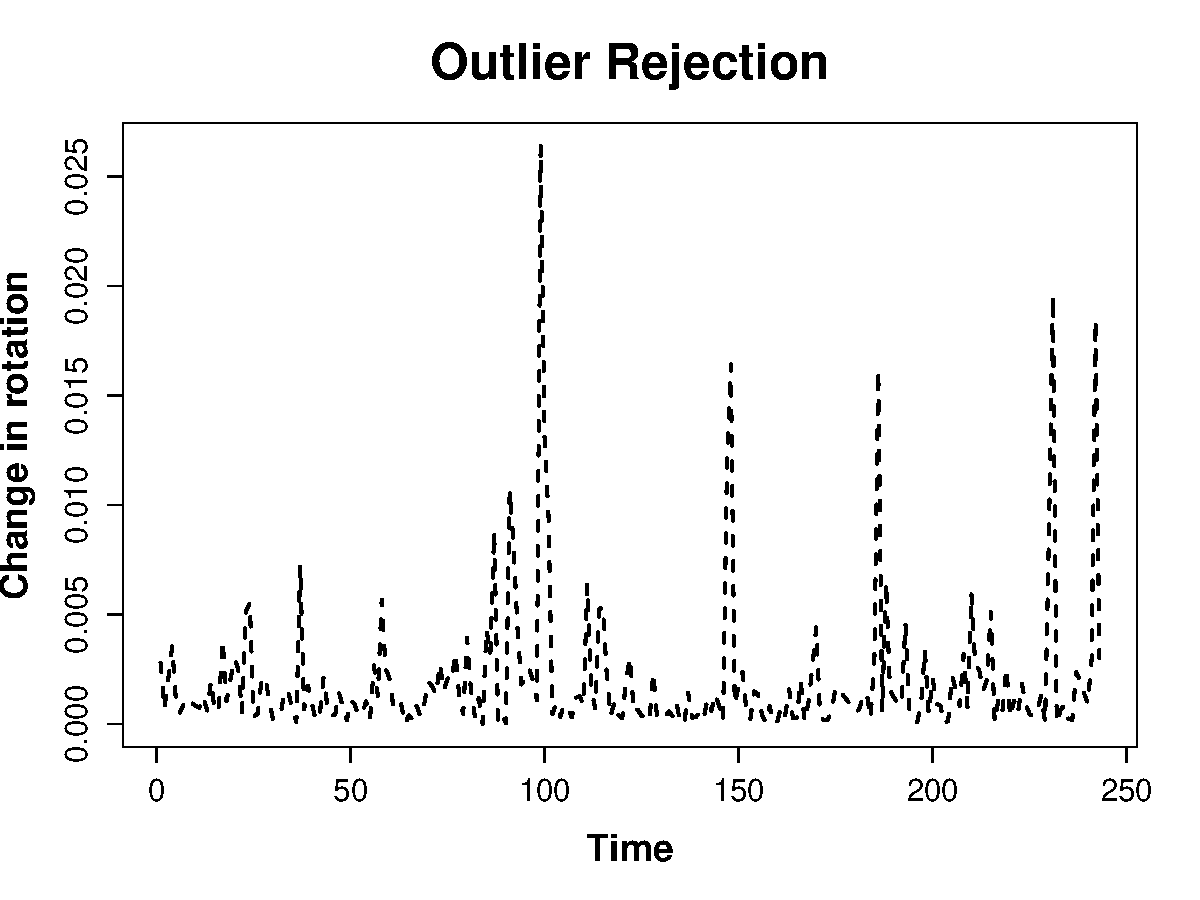
\includegraphics[width=4in]{../figures/rsfmriplot1.pdf}
\end{frame}

\begin{frame}
\frametitle{Time series / rsfMRI analysis with ANTs}
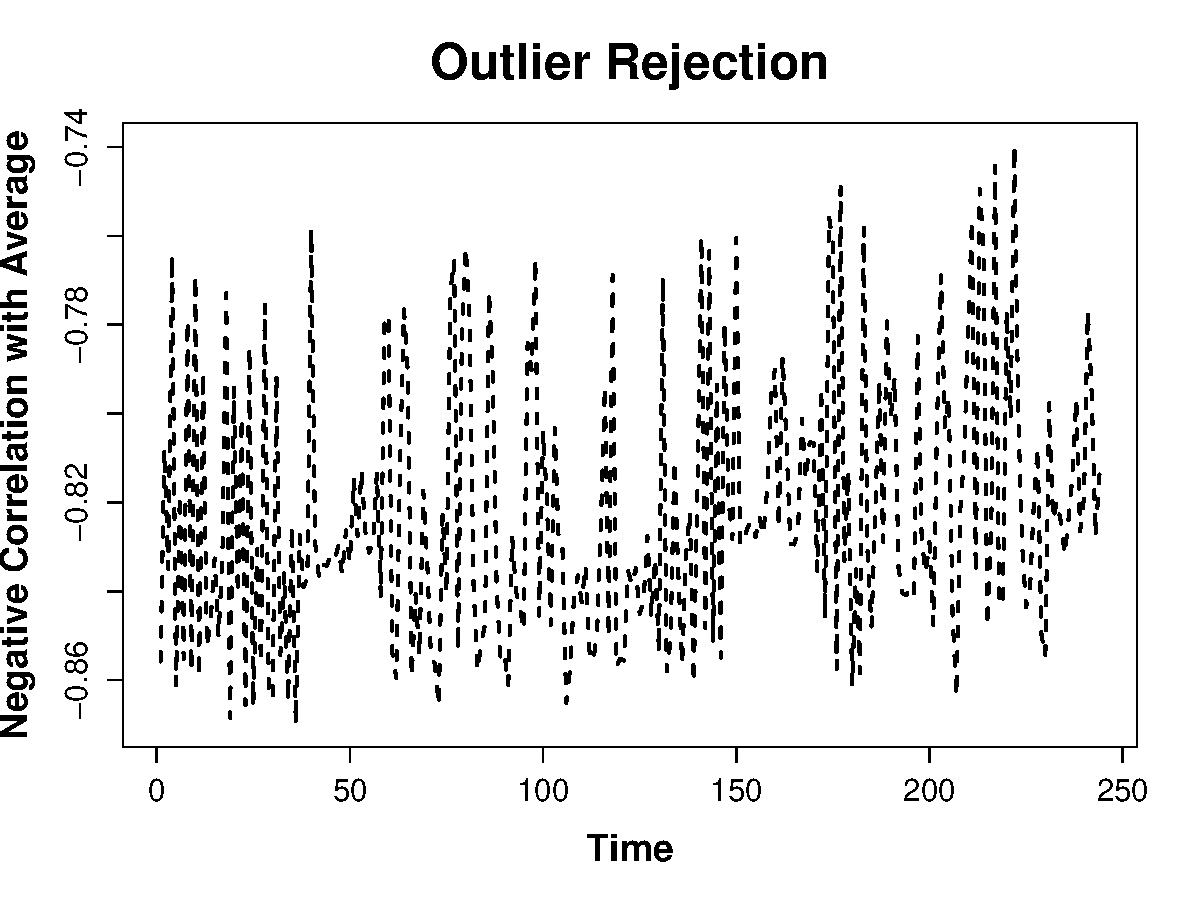
\includegraphics[width=4in]{../figures/rsfmriplot2.pdf}
\end{frame}

\begin{frame}
\frametitle{Extracting a resting state network}
   ThresholdImage 3 imgavg.nii.gz brainmask.nii.gz 1  1000 
   \newline
   \newline
   ImageMath 3 brainmask.nii.gz GetLargestComponent brainmask.nii.gz 
   \newline
   \newline
   ImageMath 4 compcorr.nii.gz CompCorrAuto motioncorrected.nii.gz   brainmask.nii.gz 6
   \newline
   \newline
%   N3BiasFieldCorrection 3 imgavg imgavg 2 brainmask 
%   \newline
%   \newline
%  Atropos -d 3 -a imgavg -a compcorr\_variance.nii.gz -m  [0.3,1x1x1] -o [seg.nii.gz,prob\_ \%02d.nii.gz] -c [5,0] -i kmeans[3] -x brainmask 
%   \newline
%   \newline
%   ThresholdImage 3 prob\_02.nii.gz cortmask.nii.gz 0.1 1.0
%     \newline
%   \newline
   sccan  --timeseriesimage-to-matrix [ motioncorrected.nii.gz,   brainmask.nii.gz, 5.0 , 0.0 ] -o out.csv 
   \newline
   \newline
   sccan  --svd sparse[ out.csv, cortmask.nii.gz, -0.05 ] -n 40 -i 40  --PClusterThresh 100  -o RSF\_Nodes.nii.gz
   \newline
   \newline
   Then build a graph ( see iGraph ).
\end{frame}


\begin{frame}
\frametitle{Statistical analysis with ANTs}
script based 
\end{frame}

\begin{frame}
\frametitle{How does structure and functional connectivity elaborate during development?}
open data
\end{frame}


\begin{frame}
\frametitle{Reproducibility}
\Huge
\begin{itemize}
\item ANTs is ideal for producing reproducible research.
\pause
\item It is multi-platform and portable.
\pause
\item It can easily be modified for $+++$ different types of studies. 
\end{itemize}
\end{frame}

\begin{frame}
\frametitle{Reproducibility}
\Huge
\begin{itemize}
\item ANTs allows one to access the powers of both ITK and {\bf
    R}. 
\pause
\item We aim to support user needs so if you can't find something,
  just ask .... Questions?
\end{itemize}
\end{frame}

\begin{frame}
\frametitle{Acknowledgements}
\Large
\begin{itemize}
\item NIBIB for software development support under grant R01-EB006266-01.
\item The ITK development team.
\item Dr. Murray Grossman for pushing application development.
\item The NLM for providing stimulus funding in support of ITKv4. 
\end{itemize}
\end{frame}



\end{document}



ants multivariate tutorial

implement with beamer : github, scripts, figures, etc

pauly:  pointset matching with b-splines 

hongzhi:  I will be interested to know how to incorporate additional information, such as landmarks, other than images to help registration, how to build atlases and do groupwise registration with ANTS

JJ data as guide + ADNI for longitudinal processing 


graph analysis

I'm most interested in relating structural images to continuous behavioral measures - for example, age, the amount of improvement on a behavioral task, or the level of some CSF analyte (I'm assuming the analysis would be essentially identical for any continuous measure...).


--- asymmetry is important 

